10. Для нахождения области определения данной функции необходимо решить неравенство\\ $\cfrac{(x-1)^2(2x-x^2+2)}{(x^2+x-6)|x+2|}\geqslant0\Leftrightarrow
\cfrac{(x-1)^2(x-(1-\sqrt{3}))(x-(1+\sqrt{3}))}{(x-2)(x+3)|x+2|}\leqslant0.$ Применив метод интервалов, найдём ответ:
\begin{figure}[ht!]
\center{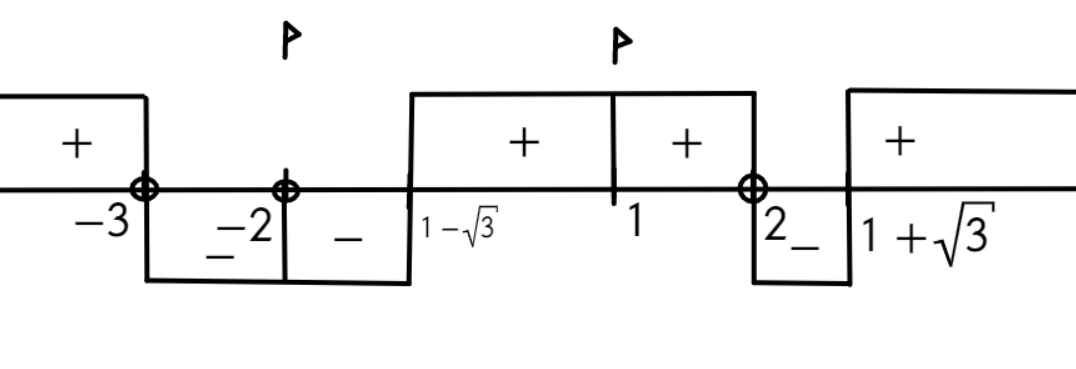
\includegraphics[scale=0.35]{isl10.png}}
\end{figure}
$x\in(-3;-2)\cup(-2;1-\sqrt{3}]\cup\{1\}\cup(2;1+\sqrt{3}].$\\
